\section{Experiments}

\subsection{Idealness experiments}

We now turn our attention to two specific compression functions, the
LZ77 and Huffman function. These two compression functions are of
interest for two reasons. First, they are representative of the way
typical lossless compression functions work internally, by taking
advantage of letter frequencies (Huffman) or letter-sequence
repetitions (LZ77). Second, they are the ones almost exclusively used in
practice. The DEFLATE algorithm \cite{deutsch1996deflate}, which is a composition of LZ77 and
Huffman, is the algorithm used in gzip, which is prevalent on the
modern web. In 2016, 98.85\% of websites that enabled compression used
some form of gzip. We argue that both LZ77 and Huffman are nearly
ideal compression functions. The complexity of the Huffman and
especially the LZ77 algorithms arises from many intricate technical
details, such as, for instance, the sliding window size of LZ77. These
details make it impractical to deal with these functions in analytical
proofs.

We support our idealness claims in an experimental manner. Our experiment
measured the compression performance of the Huffman and an ideal function on a
text of English literature\footnote{The screenplay of the movie ``The Social
Network".}. First, we calculated the occurences of each character (letters and
digits) in the text. Second, we generated the Huffman
table for this text and the table of an ideal function based on the character
frequencies. Each character is represented by a bitstream in both tables. Figure
\ref{fig:huffman_idealness} depicts the length of the bitstreams of characters
in descending order of occurencies for both the ideal and the Huffman functions.

    \begin{figure}[thpb]
        \centering
            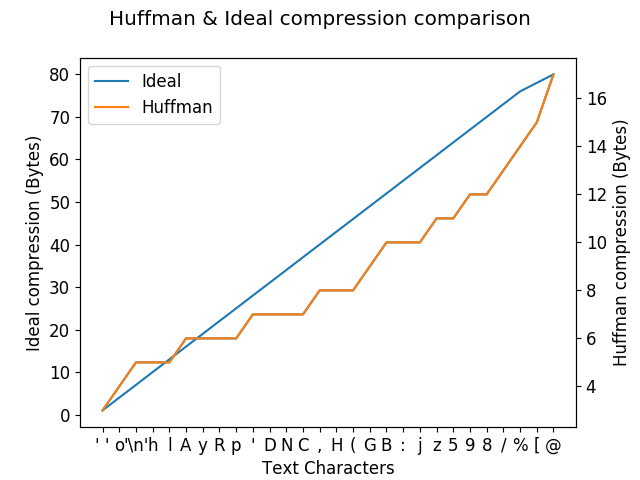
\includegraphics[width=0.48\textwidth]{experiments/huffman_idealness/huffman_idealness.png}
        \caption{Huffman-ideal compression comparison}
        \label{fig:huffman_idealness}
    \end{figure}

